% Made up for the tikra benchmark.
\usetikzlibrary{shapes.geometric}
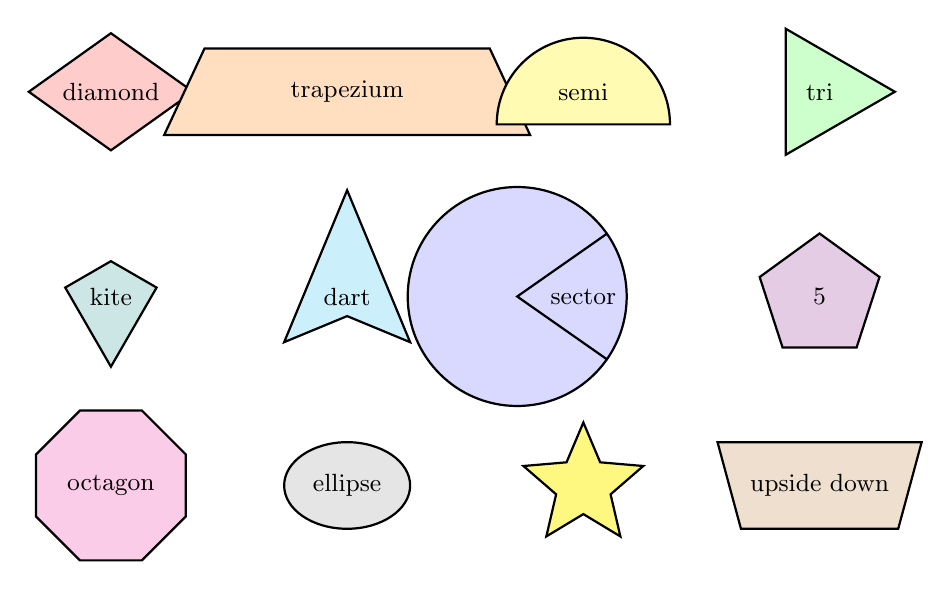
\begin{tikzpicture}[base/.style={draw, thick, minimum width=1.6cm, minimum height=1.1cm, font=\small}]
  \node[base, diamond, fill=red!20, aspect=1.4] at (0,0) {diamond};
  \node[base, trapezium, trapezium left angle=65, trapezium right angle=65, fill=orange!25] at (3,0) {trapezium};
  \node[base, semicircle, fill=yellow!30] at (6,0) {semi};
  \node[base, isosceles triangle, isosceles triangle apex angle=60, fill=green!20] at (9,0) {tri};
  \node[base, kite, fill=teal!20, minimum width=1.1cm] at (0,-2.6) {kite};
  \node[base, dart, fill=cyan!20, shape border rotate=90] at (3,-2.6) {dart};
  \node[base, circular sector, circular sector angle=70, shape border rotate=180, fill=blue!15] at (6,-2.6) {sector};
  \node[base, regular polygon, regular polygon sides=5, fill=violet!20] at (9,-2.6) {5};
  \node[base, regular polygon, regular polygon sides=8, fill=magenta!20] at (0,-5) {octagon};
  \node[base, ellipse, fill=gray!20] at (3,-5) {ellipse};
  \node[base, star, star points=5, star point ratio=2.2, fill=yellow!50] at (6,-5) {};
  \node[base, trapezium, trapezium stretches body, shape border rotate=180, fill=brown!25, minimum width=2cm] at (9,-5) {upside down};
\end{tikzpicture}
